\section{条件分布的计算}
\label{sec:rvc-conditional}

第一台传感器读到$0$，第二台会读什么？已经知道$X=0$，所有$X\neq0$的样本点都被排除，剩下的只有概率表的第一行。第~\ref{chap:classical-probability}章的条件概率正是这样做的：缩小样本范围，再把剩下的质量重新归一，使总和回到$1$。这一节把这个操作用到联合分布上，先在概率表中计算，再处理密度，最后用条件分布计算条件均值，并把总方差拆成两部分。

\paragraph{概率表中的条件分布}
设$p_X(x)>0$。由条件概率的定义，
\[
 \mathbb{P}(Y=y\mid X=x)=\frac{\mathbb{P}(X=x,\,Y=y)}{\mathbb{P}(X=x)}.
\]
把它看作$y$的函数，记
\begin{equation}
 p_{Y\mid X}(y\mid x)=\frac{p_{X,Y}(x,y)}{p_X(x)},\qquad p_X(x)>0 ,
 \label{eq:rvc-conditional-pmf}
\end{equation}
称为给定$X=x$时$Y$的\term{条件质量函数}（conditional probability mass function），它确定的分布称为给定$X=x$时$Y$的\term{条件分布}（conditional distribution）。对固定的$x$，分子按$y$求和恰好是分母，所以条件质量函数非负且和为$1$，是一个正常的概率表。

在概率表上，这就是取出第$x$行，再除以该行之和。传感器表的三行之和分别为$0.3,0.4,0.3$，得到
\[
 p_{Y\mid X}(\cdot\mid 0)=\bigl(\tfrac23,\tfrac13,0\bigr),\quad
 p_{Y\mid X}(\cdot\mid 1)=\bigl(\tfrac14,\tfrac12,\tfrac14\bigr),\quad
 p_{Y\mid X}(\cdot\mid 2)=\bigl(0,\tfrac13,\tfrac23\bigr).
\]
第一台读$0$时，第二台不可能读$2$；第一台读$1$时，第二台的读数对称地分布在$1$两侧。三行的形状互不相同，见图~\ref{fig:rvc-conditional-pmf}。

\begin{BookInlineFigure}
  \centering
  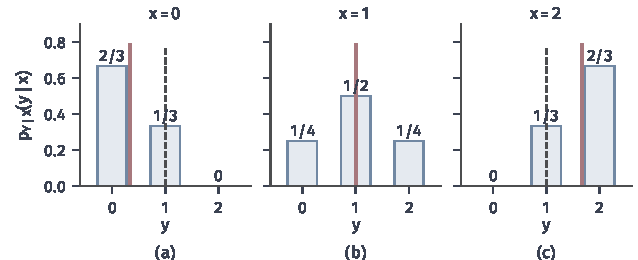
\includegraphics[width=108mm]{figures/07-probability/01-elementary-probability/matplotlib/rvc-conditional-pmf/figure.pdf}
  \caption{传感器表中给定第一台读数时第二台读数的条件分布。(a)、(b)、(c)分别对应$x=0,1,2$，柱高为$p_{Y\mid X}(y\mid x)$；红线是条件均值$1/3$、$1$、$5/3$，虚线是不加条件时的均值$1$。}
  \label{fig:rvc-conditional-pmf}
\end{BookInlineFigure}

把式~\eqref{eq:rvc-conditional-pmf}两边乘以$p_X(x)$，得到联合质量的另一种写法：
\begin{equation}
 p_{X,Y}(x,y)=p_X(x)\,p_{Y\mid X}(y\mid x).
 \label{eq:rvc-multiplication}
\end{equation}
它说明联合分布可以分两步给出：先按$p_X$定下$X$的值，再按该值对应的条件分布定下$Y$。许多模型正是这样描述的，先说明一个量怎样产生，再说明另一个量在前者给定时怎样产生。对$x$求和就是第~\ref{chap:classical-probability}章的全概率公式，
\[
 p_Y(y)=\sum_{x}p_X(x)\,p_{Y\mid X}(y\mid x),
\]
其中$p_X(x)=0$的项本来就是零，可以略去。反过来求给定$Y=y$时$X$的条件分布，就是Bayes公式：当$p_Y(y)>0$时，
\[
 p_{X\mid Y}(x\mid y)=\frac{p_X(x)\,p_{Y\mid X}(y\mid x)}{p_Y(y)}.
\]
传感器表关于对角线对称，例如$p_{X\mid Y}(0\mid 0)=0.3\cdot\frac23/0.3=\frac23$，与$p_{Y\mid X}(0\mid 0)$相同。

\paragraph{给连续变量取条件}
三角形模型中，若已知$X=0.6$，$Y$怎样分布？困难在于$\mathbb{P}(X=0.6)=0$，式~\eqref{eq:rvc-conditional-pmf}的分母为零。自然的办法是先以一个有正概率的窄带代替这个点：给定$x\leq X\leq x+h$，再让$h\to0$，见图~\ref{fig:rvc-conditional-slices}(a)。

设$f_{X,Y}$在$x$附近连续，且$f_X(x)>0$。窄带上的条件概率是两个积分之比，
\[
 \mathbb{P}(Y\leq y\mid x\leq X\leq x+h)
 =\frac{\int_{x}^{x+h}\int_{-\infty}^{y}f_{X,Y}(s,t)\,\mathrm{d}t\,\mathrm{d}s}{\int_{x}^{x+h}f_X(s)\,\mathrm{d}s}.
\]
分子分母同除以$h$。窄带越来越窄时，两者分别趋于被积函数在$s=x$处的值，于是
\[
 \lim_{h\to0}\mathbb{P}(Y\leq y\mid x\leq X\leq x+h)=\int_{-\infty}^{y}\frac{f_{X,Y}(x,t)}{f_X(x)}\,\mathrm{d}t .
\]
右边被积的函数正是窄带极限下$Y$的密度。

\begin{definition}[条件密度]
\label{def:rvc-conditional-density}
设$(X,Y)$有联合密度$f_{X,Y}$，$X$的边缘密度为$f_X$。对满足$f_X(x)>0$的$x$，定义
\begin{equation}
 f_{Y\mid X}(y\mid x)=\frac{f_{X,Y}(x,y)}{f_X(x)},
 \label{eq:rvc-conditional-density}
\end{equation}
称为给定$X=x$时$Y$的\term{条件密度}（conditional density）。
\end{definition}

和概率表一样，条件密度是联合密度沿竖线$\{X=x\}$的切片，除以切片的总积分$f_X(x)$而得到；它对$y$的积分为$1$。三角形模型中，对$0<x\leq1$有$f_X(x)=2x>0$，切片在$0\leq y\leq x$上取值$2$，所以
\[
 f_{Y\mid X}(y\mid x)=\frac{2}{2x}=\frac1x,\qquad 0\leq y\leq x .
\]
给定$X=x$时，$Y$服从$\operatorname{Unif}(0,x)$：均匀分布的点落在竖线上，只能落在三角形内的那一段，并且在这一段上没有偏好。

\begin{BookInlineFigure}
  \centering
  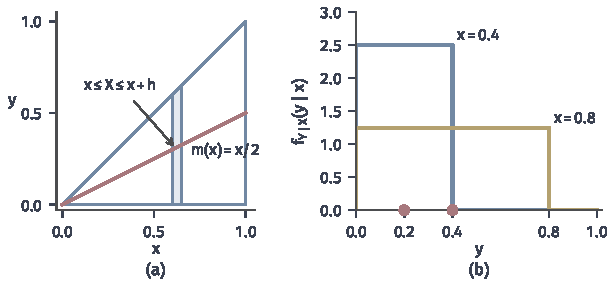
\includegraphics[width=104mm]{figures/07-probability/01-elementary-probability/matplotlib/rvc-conditional-slices/figure.pdf}
  \caption{三角形模型的条件化。(a)浅蓝窄带是事件$\{x\leq X\leq x+h\}$，$x=0.6$，$h=0.05$；红线是条件均值$m(x)=x/2$。(b)给定$X=0.4$（蓝）与$X=0.8$（黄）时$Y$的条件密度，分别是高$2.5$与$1.25$的矩形；红点是两个条件均值$0.2$与$0.4$。}
  \label{fig:rvc-conditional-slices}
\end{BookInlineFigure}

式~\eqref{eq:rvc-conditional-density}只在$f_X(x)>0$处使用。另一个限制更隐蔽：联合密度可以在一条竖线$\{x=x_0\}$上任意改动而不改变任何概率，改动后$f_{Y\mid X}(\cdot\mid x_0)$就变了。所以单独一个$x_0$处的条件密度并不由联合分布决定；只有把各个$x$处的条件密度合起来使用，例如对$x$积分，结果才有确定的意义。条件于零概率事件的严格含义，以及不同的取极限方式可能给出不同答案的现象，在第~\ref{chap:conditional-distributions}章说明。

有了条件密度，式~\eqref{eq:rvc-multiplication}和全概率公式都有连续版本：在$f_X(x)>0$处$f_{X,Y}(x,y)=f_X(x)f_{Y\mid X}(y\mid x)$，并且
\[
 f_Y(y)=\int f_X(x)\,f_{Y\mid X}(y\mid x)\,\mathrm{d}x,
\]
积分只在$f_X(x)>0$的范围进行。对三角形模型，$\int_{y}^{1}2x\cdot\frac1x\,\mathrm{d}x=2(1-y)$，与第~\ref{sec:rvc-joint}节直接求出的$f_Y$相同。

反方向的条件化同样计算。给定$Y=y$，$0\leq y<1$，由$f_Y(y)=2(1-y)>0$，
\[
 f_{X\mid Y}(x\mid y)=\frac{2}{2(1-y)}=\frac{1}{1-y},\qquad y\leq x\leq 1 ,
\]
即$X$在给定$Y=y$时服从$\operatorname{Unif}(y,1)$：较小的读数已知为$y$，较大的读数在$y$与$1$之间没有偏好。横线与竖线上的切片都是均匀的，但切片的位置与长度随条件改变，这正是两个分量不独立的表现。

\paragraph{条件分布与独立}
独立性可以换一种方式理解：知道$X$的值不改变$Y$的分布。在概率表的情形，由式~\eqref{eq:rvc-independence-pmf}与式~\eqref{eq:rvc-conditional-pmf}，$X,Y$独立当且仅当对每个满足$p_X(x)>0$的$x$，
\[
 p_{Y\mid X}(y\mid x)=p_Y(y)\quad\text{对一切}\ y\ \text{成立}.
\]
条件分布与$x$无关，各行重新归一以后长得一样。传感器表的三行形状各异，再次说明两台读数不独立。

有密度时，若$X,Y$独立，取$f_Xf_Y$为联合密度，条件密度就是$f_Y$，同样与$x$无关。图~\ref{fig:rvc-slices}比较了两个连续模型：$f=4xy$的条件密度在三个$x$处完全重合，都是$2y$；三角形模型的条件密度是宽度为$x$的矩形，随$x$改变。

\begin{BookInlineFigure}
  \centering
  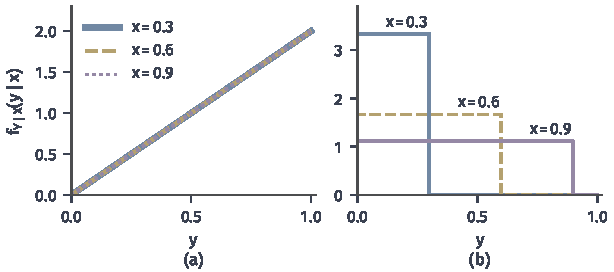
\includegraphics[width=104mm]{figures/07-probability/01-elementary-probability/matplotlib/rvc-slices/figure.pdf}
  \caption{独立就是条件分布不随条件改变。蓝、黄、紫分别对应$x=0.3,0.6,0.9$。(a)单位正方形上的密度$4xy$，三条条件密度重合为$2y$。(b)三角形模型，条件密度是$[0,x]$上高为$1/x$的矩形。}
  \label{fig:rvc-slices}
\end{BookInlineFigure}

\paragraph{离散状态与连续读数}
条件变量与被条件变量不必同属一类。设房间有两种状态：$X=0$表示正常，$X=1$表示过热，$\mathbb{P}(X=1)=0.2$。正常时一台精确传感器的读数$Y$服从$\mathcal{N}(20,1)$，过热时服从$\mathcal{N}(23,1)$。这里$X$有概率表，$Y$在给定$X$时有密度，联合规律由式~\eqref{eq:rvc-multiplication}的两步方式给出：
\begin{equation}
 \mathbb{P}(X=x,\,Y\in B)=p_X(x)\int_{B}f_{Y\mid X}(y\mid x)\,\mathrm{d}y .
 \label{eq:rvc-mixed-joint}
\end{equation}

对$x$求和，$Y$的边缘密度是两个高斯密度的加权和。记$\phi(z)=\mathrm{e}^{-z^{2}/2}/\sqrt{2\pi}$为标准高斯密度，则
\[
 f_Y(y)=0.8\,\phi(y-20)+0.2\,\phi(y-23).
\]
这种由若干分布按权重相加得到的分布称为\term{混合分布}（mixture distribution）。图~\ref{fig:rvc-mixture}(a)中，蓝线是$f_Y$，主峰来自正常状态，右侧的肩来自过热状态。

\begin{BookInlineFigure}
  \centering
  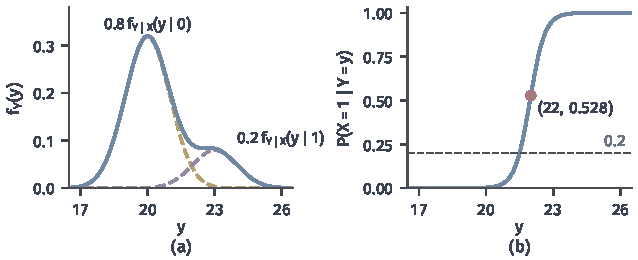
\includegraphics[width=108mm]{figures/07-probability/01-elementary-probability/matplotlib/rvc-mixture/figure.pdf}
  \caption{离散状态与连续读数。$\mathbb{P}(X=1)=0.2$，给定$X=0$与$X=1$时$Y$分别服从$\mathcal{N}(20,1)$与$\mathcal{N}(23,1)$。(a)蓝线为$Y$的密度，黄、紫虚线为两部分$0.8\,\phi(y-20)$与$0.2\,\phi(y-23)$。(b)读到$y$以后过热的条件概率，虚线是不加条件时的概率$0.2$，红点为$y=22$。}
  \label{fig:rvc-mixture}
\end{BookInlineFigure}

读到$Y=y$以后，过热的可能性有多大？$\mathbb{P}(Y=y)=0$，仍用窄带$y\leq Y\leq y+h$取极限，由式~\eqref{eq:rvc-mixed-joint}，分子分母同除以$h$后得到Bayes公式的密度形式：
\begin{equation}
 \mathbb{P}(X=1\mid Y=y)=\frac{p_X(1)\,f_{Y\mid X}(y\mid 1)}{f_Y(y)} .
 \label{eq:rvc-mixed-bayes}
\end{equation}
取$y=22$，两部分分别含$\phi(-1)$与$\phi(2)$，约去$1/\sqrt{2\pi}$，
\[
 \mathbb{P}(X=1\mid Y=22)=\frac{0.2\,\mathrm{e}^{-1/2}}{0.2\,\mathrm{e}^{-1/2}+0.8\,\mathrm{e}^{-2}}
 =\frac{1}{1+4\mathrm{e}^{-3/2}}\approx0.528 .
\]
读数$22$离过热状态的中心更近，过热的概率从$0.2$升到一半以上。取$y=21.5$时，两部分的指数相同，比值回到先验权重：$\mathbb{P}(X=1\mid Y=21.5)=0.2$，这个读数不提供区分两种状态的信息。

\paragraph{条件均值}
条件分布确定以后，可以像一元情形一样求它的期望。设$\mathbb{E}\lvert Y\rvert<\infty$，并且下面的和或积分有限，定义
\begin{equation}
 m(x)=\mathbb{E}[Y\mid X=x]=\sum_{y}y\,p_{Y\mid X}(y\mid x)\quad\text{或}\quad\int y\,f_{Y\mid X}(y\mid x)\,\mathrm{d}y ,
 \label{eq:rvc-conditional-mean}
\end{equation}
称为给定$X=x$时$Y$的\term{条件均值}（conditional mean）。它是“只看$X=x$那一组”时$Y$的平均，即组内平均。

传感器表中，由三行条件分布，
\[
 m(0)=\tfrac13,\qquad m(1)=1,\qquad m(2)=\tfrac53 ,
\]
可以合写为$m(x)=1/3+2x/3$。三角形模型中$Y$在给定$X=x$时服从$\operatorname{Unif}(0,x)$，$m(x)=x/2$。有趣的是，两个例子中$m$恰好都等于式~\eqref{eq:rvc-best-line}的最佳直线$\mu_Y+b^{*}(x-\mu_X)$：传感器表中$b^{*}=0.4/0.6=2/3$，三角形模型中$b^{*}=(1/36)/(1/18)=1/2$。一般情形下条件均值不必是直线，它作为最佳预测的含义在第~\ref{chap:conditional-expectation}章说明。

把$x$换成随机的$X$，得到随机变量$m(X)$，记作$\mathbb{E}[Y\mid X]$。它的值随$X$的值而定：传感器表中，$\mathbb{E}[Y\mid X]$以概率$0.3,0.4,0.3$取$1/3,1,5/3$。它的期望回到$Y$的期望，这就是下面的\term{全期望公式}（law of total expectation）。

\begin{theorem}[全期望公式]
\label{thm:rvc-total-expectation}
设$\mathbb{E}\lvert Y\rvert<\infty$，$X$有概率表或$(X,Y)$有联合密度。则
\begin{equation}
 \mathbb{E}[Y]=\mathbb{E}\bigl[\mathbb{E}[Y\mid X]\bigr]=\sum_{x}m(x)\,p_X(x)\quad\text{或}\quad\int m(x)\,f_X(x)\,\mathrm{d}x .
 \label{eq:rvc-total-expectation}
\end{equation}
\end{theorem}

\begin{proof}
在概率表的情形，由式~\eqref{eq:rvc-multiplication}，
\[
 \sum_{x}p_X(x)\,m(x)=\sum_{x}p_X(x)\sum_{y}y\,p_{Y\mid X}(y\mid x)=\sum_{x,y}y\,p_{X,Y}(x,y).
\]
条件$\mathbb{E}\lvert Y\rvert<\infty$保证二重和绝对收敛，求和可以按任意分组进行，右边就是$\mathbb{E}[Y]$。在密度的情形，把求和换成积分，并在$f_X(x)>0$处使用$f_{X,Y}=f_Xf_{Y\mid X}$。
\end{proof}

全期望公式就是“总平均等于各组平均的加权平均”，权重是各组的质量。传感器表中，
\[
 0.3\cdot\tfrac13+0.4\cdot1+0.3\cdot\tfrac53=0.1+0.4+0.5=1=\mathbb{E}[Y].
\]
三角形模型中，两个方向的条件均值分别是$m(x)=x/2$与$\mathbb{E}[X\mid Y=y]=(1+y)/2$，代入全期望公式，
\[
 \mathbb{E}[Y]=\frac{\mathbb{E}[X]}{2}=\frac13,\qquad \mathbb{E}[X]=\frac{1+\mathbb{E}[Y]}{2}=\frac23,
\]
都与边缘密度算出的结果一致。混合模型中$\mathbb{E}[Y]=0.8\cdot20+0.2\cdot23=20.6$。

\paragraph{全方差公式}
条件分布也有方差。设$\mathbb{E}[Y^{2}]<\infty$，在概率表的情形定义
\begin{equation}
 v(x)=\operatorname{Var}(Y\mid X=x)=\sum_{y}\bigl(y-m(x)\bigr)^{2}p_{Y\mid X}(y\mid x),
 \label{eq:rvc-conditional-variance}
\end{equation}
称为给定$X=x$时$Y$的\term{条件方差}（conditional variance）；密度的情形把和换成积分。它是组内的散开程度。$Y$的总方差与它有什么关系？回答是下面的\term{全方差公式}（law of total variance）。

\begin{theorem}[全方差公式]
\label{thm:rvc-total-variance}
设$\mathbb{E}[Y^{2}]<\infty$，$X$有概率表或$(X,Y)$有联合密度。则
\begin{equation}
 \operatorname{Var}(Y)=\mathbb{E}\bigl[v(X)\bigr]+\operatorname{Var}\bigl(m(X)\bigr).
 \label{eq:rvc-total-variance}
\end{equation}
\end{theorem}

\begin{proof}
记$\mu_Y=\mathbb{E}[Y]$，在概率表的情形证明。固定满足$p_X(x)>0$的$x$，把$y-\mu_Y$拆成$(y-m(x))+(m(x)-\mu_Y)$，在条件分布下求平方的平均。交叉项含有$\sum_{y}(y-m(x))p_{Y\mid X}(y\mid x)$，由$m(x)$的定义它等于零，于是
\[
 \sum_{y}(y-\mu_Y)^{2}p_{Y\mid X}(y\mid x)=v(x)+\bigl(m(x)-\mu_Y\bigr)^{2}.
\]
两边乘以$p_X(x)$再对$x$求和。由式~\eqref{eq:rvc-multiplication}，左边成为
\[
 \sum_{x,y}(y-\mu_Y)^{2}p_{X,Y}(x,y)=\operatorname{Var}(Y).
\]右边第一项是$\mathbb{E}[v(X)]$；由全期望公式$\mathbb{E}[m(X)]=\mu_Y$，第二项是$\operatorname{Var}(m(X))$。密度的情形逐字把求和换成积分。
\end{proof}

证明中的第一个等式是力学中的平行轴定理：质量对任意一点的二阶矩，等于对自身重心的二阶矩加上重心偏移的平方。式~\eqref{eq:rvc-total-variance}于是读作：总波动等于组内波动的平均，加上各组平均之间的波动。

三个例子逐一核对。传感器表中三行的条件方差为$2/9,1/2,2/9$，$m(X)=1/3+2X/3$，所以
\[
 \mathbb{E}[v(X)]=0.3\cdot\tfrac29+0.4\cdot\tfrac12+0.3\cdot\tfrac29=\tfrac13,\qquad
 \operatorname{Var}\bigl(m(X)\bigr)=\bigl(\tfrac23\bigr)^{2}\cdot0.6=\tfrac{4}{15},
\]
两者之和为$9/15=0.6=\operatorname{Var}(Y)$。三角形模型中$v(x)=x^{2}/12$，$m(X)=X/2$，
\[
 \mathbb{E}[v(X)]=\frac{\mathbb{E}[X^{2}]}{12}=\frac{1}{24},\qquad
 \operatorname{Var}\bigl(m(X)\bigr)=\frac{\operatorname{Var}(X)}{4}=\frac{1}{72},
\]
和为$1/18$。混合模型中两组的方差都是$1$，组平均$20$与$23$以权重$0.8,0.2$分布，组间方差为$3^{2}\times0.8\times0.2=1.44$，所以$\operatorname{Var}(Y)=1+1.44=2.44$。

由式~\eqref{eq:rvc-total-variance}，$\mathbb{E}[v(X)]\leq\operatorname{Var}(Y)$：平均而言，知道$X$以后$Y$的不确定性不会增加。但这只对平均成立，个别条件可以让波动变大。单位圆盘的均匀分布中，$\operatorname{Var}(Y)=\mathbb{E}[Y^{2}]=1/4$，而给定$X=0$时$Y$服从$\operatorname{Unif}(-1,1)$，条件方差为$1/3$；圆盘中央那条竖线比整个圆盘在竖直方向更“长”。

本节的计算都针对给定的具体取值$x$，结果是$x$的普通函数。把条件均值当作随机变量来研究，例如它为什么是在已知$X$时对$Y$的最佳预测、在什么意义下唯一，属于第~\ref{chap:conditional-expectation}章；没有概率表也没有密度时怎样定义条件分布，属于第~\ref{chap:conditional-distributions}章。
